\section{Model from Template protocol}
\label{app:modelFromTemplate}%a110
Protocol designed to obtain a structure model for a target sequence in \scipion. Target structure is predicted by sequence homology using \modeller \citep{sali1993} web service in \chimera.\\
WARNING: Working with \modeller requires a license key, which can be requested free of charge for academic users. Try to have this license key before starting the protocol execution. 

   
 \begin{itemize}
  \item Requirements to run this protocol and visualize results:
            \begin{itemize}
                \item \scipion plugin: \ttt{scipion-em}
                \item \scipion plugin: \ttt{scipion-em-chimera}
                \item Multiple sequence alignment tools: \ttt{Clustal Omega}, \ttt{MUSCLE}
            \end{itemize}
  \item \scipion menu:
            \ttt{Model building -> Initial model} (\ffigure{fig:app_protocol_seqHomology_1} (A))
  
  \item Protocol form parameters (\ffigure{fig:app_protocol_seqHomology_1} (B)):
  
            \begin{figure}[H]
                \centering 
                \captionsetup{width=.9\linewidth} 
                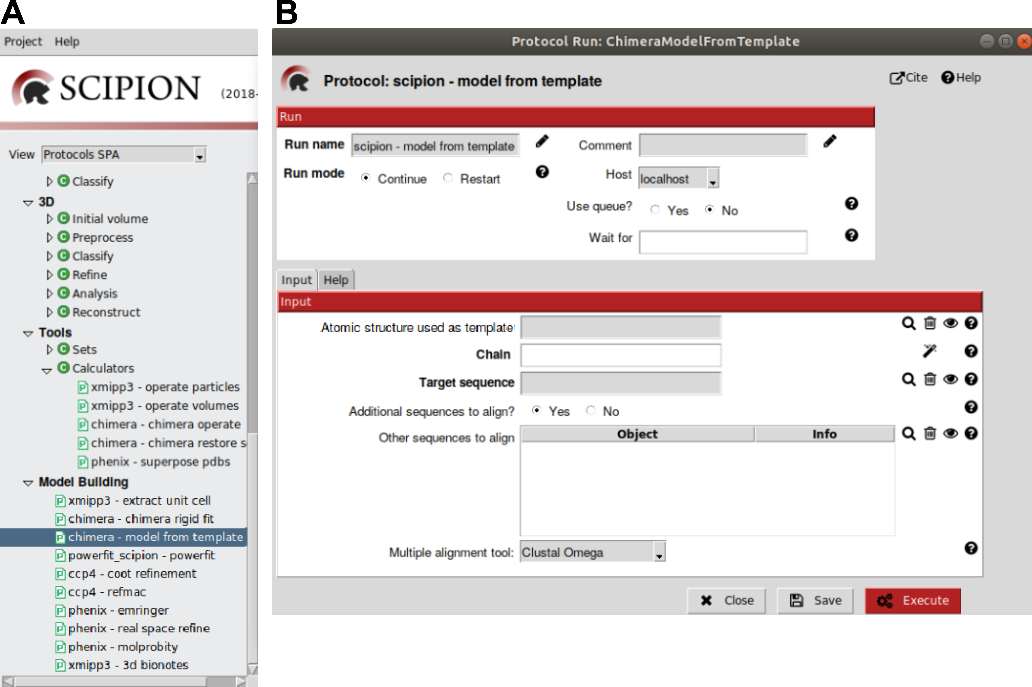
\includegraphics[width=0.90\textwidth]{Images_appendix/Fig111.pdf}
                \caption{Protocol \scommand{model from template}. A: Protocol location in \scipion menu. B: Protocol form: Option ``template available''. C: Protocol form: Option ``looking for template''.}
                \label{fig:app_protocol_seqHomology_1}
            \end{figure}
            
            \begin{itemize}
                    \item \ttt{Input} section
  

                        \begin{itemize}
                        \item \ttt{Do you already have a template?}: Select \ttt{``Yes''} if you have found your \iii{template} in a previous similarity searching step. Select \ttt{``No''} if you do not have any \iii{template} to start the homology modeling and you would like to search for one.
                        \item Option \ttt{``Yes''} (\ffigure{fig:app_protocol_seqHomology_1} (B))
                                        \begin{itemize}
                                                \item \ttt{Atomic structure used as template}: Atomic structure previously downloaded in \scipion. This structure was selected by sequence homology, i.e. by looking for the structurally characterized sequence more similar (with higher identity) to the target sequence.
                                                \item \ttt{Chain}: Specific monomer of the macromolecule that has to be used as structure \iii{template} of the \ttt{target sequence}. Use the wizard on the right side of \ttt{Chain} parameter to select that chain.
                                                \item \ttt{Target sequence}: Sequence previously downloaded in \scipion. This sequence has to be modeled following the structure skeleton of the selected \iii{template}.
                                                \item \ttt{Options to improve the alignment}: $Modeller$ provides structural models of the \iii{target sequence} based on a sequence alignment, in which at least sequences of \iii{template} and \iii{target} have to be included. Three options can be considered to improve this alignment:
                                                \begin{enumerate}
                                                \item \ttt{None}: No more sequences are going to be included in the alignment except \iii{model} and \iii{target} sequences. Correlative param:\\
                                                     *** \ttt{Alignment tool for two sequences}: Select one of the three available alignment methods, \ttt{Bio.parirwise2} (by default), \ttt{Clustal Omega}, \ttt{MUSCLE}.
                                                \item \ttt{Additional sequences to align} if you want to perform a multiple sequence alignment adding other sequences already downloaded in \scipion. Additional sequences, others than \ttt{template} and \ttt{target} sequences, are required to accomplish this multiple alignment. Correlative params:\\
                                                     *** \ttt{Other sequences to align}: Box to complete with the additional sequences used to perform the multiple sequence alignment. All of them were previously downloaded in \scipion.\\
                                                     *** \ttt{Multiple alignment tool}: Select between \ttt{Clustal Omega} and \ttt{MUSCLE} methods.
                                                \item \ttt{Provide your own sequence alignment}: If you want to include other sequences in the alignment by providing your own sequence alignment. Correlative param:\\
                                                    *** \ttt{Sequence alignment input}: Complete this box with the help of the right side browser including the sequence alignment file that you already have saved in your computer. Different alignment formats are available (\url{https://www.cgl.ucsf.edu/chimerax/docs/user/commands/open.html}). An example of alignment in \ttt{fasta} format can be seen below (Use case 3).
                                                \end{enumerate}
                                                \item \ttt{Additional target sequence to include?}: Select \ttt{``Yes''} if you'd like to obtain a multimer \iii{model} by using two \iii{target} sequences and the same multimer \iii{template}. The params to complete the option \ttt{``Yes''} are identical to those already shown, with the exception of the \ttt{Atomic structure used as template}, already completed. However, no one of those params will appear in case you select \ttt{``No''} in order to obtain a \iii{model} by using only one \iii{target} sequence.
                                        \end{itemize}
                        \item Option \ttt{``No''} (\ffigure{fig:app_protocol_seqHomology_1} (C)) 
                                        \begin{itemize}
                                                \item \ttt{Target sequence}: Sequence previously downloaded in \scipion. This sequence has to be modeled following the structure skeleton of the \iii{template} that you are going to select among the retrieved entries found by the similarity searching tool.
                                                \item \ttt{Protein sequence database}: Select one of the two suggested protein sequence databases, PDB and NR. Press the \ttt{``?''} symbol on the right to see the meaning of each one. Remark that the NR database allows you to get entries with as well as without atomic structure associated. These ones, which do not provide \iii{templates}, could be useful to build a better sequence alignment.
                                                \item \ttt{Similarity matrix}: Select one of the ``substitution matrix'' to assign a score to any couple of residues in the alignment (\url{https://www.ncbi.nlm.nih.gov/blast/html/sub_matrix.html}).
                                                \item \ttt{cutoff evalue}: Maximum statistic value required to include a retrieved element in the hit list.
                                                \item \ttt{Maximum number of sequences} that you'd like to retrieve from the database. 
                                        \end{itemize}
                        \end{itemize}
                
                \item \ttt{Help} section
  
  Follow this section steps to run $Modeller$ via web service in \chimera and to select and save one of the retrieved models in \scipion framework.
  
  \end{itemize}
  \item Protocol execution:
  
  Adding specific template-target label is recommended in \ttt{Run name} section, at the form top. To add the label, open the protocol form, press the pencil symbol on the right side of \ttt{Run name} box, complete the label in the new opened window, press OK and, finally, close the protocol. This label will be shown in the output summary content (see below). If you want to run again this protocol, do not forget to set to \ttt{Restart} the \ttt{Run mode}.\\
  Press the \ttt{Execute} red button at the form bottom.\\
  
  Several \chimera windows will be opened after executing the protocol with different contents according to the distinct form param options. Although we are going to detail some of them through several use cases (see below), designed to ilustrate different applications of this protocol, as well as the procedure to follow in each case, in general we can predict the opening of \chimera graphics window and a sequence alignment window. Usually, in both windows the \iii{template} sequence is green highlighted (see an example of these windows in \ffigure{fig:chimera_alignment}). Main steps to follow ahead are:
            \begin{itemize}
            \item Ask for model(s) to $Modeller$ by selecting \ttt{Tools -> Sequence -> Modeller Comparative} in the main menu of \chimera graphics window. 
            \item Complete the new window opened for \ttt{Modeller Comparative} with the sequence alignment that includes the \iii{template} and with the \iii{target}(s) sequence(s), $Modeller$ license key, multichain model, number of models retrieved by \modeller, and \ttt{Advanced} options like the building of models with hydrogens, as well as $model$ inclusion of heteroatoms or water molecules. An example of completed $Modeller$ window can be observed in \ffigure{fig:modeller} (A). By pressing \ttt{OK} the computation starts. The status of the job can be checked in the lower left corner of \chimera graphics window.
            \item After a while a new panel window will show retrieved models of the \ttt{target} sequence (\ffigure{fig:modeller} (B)). Two statistics assess these models: \ttt{GA341}, statistical potentials derived-score, and \ttt{zDOPE}, normalized Discrete Optimized Protein Energy, atomic distance depending-score. Reliable models show \ttt{GA341} values higher than 0.7, and negative \ttt{zDOPE} values correspond to better models.  Retrieved models can be checked in \chimera \ttt{Tools -> Models}. One of them should be selected (\ffigure{fig:modeller} (C)).
            \item Rename the selected model, for example \ttt{\#n\_initial} to \ttt{\#n\_final} with the command line:\\ \ttt{rename \#n\_initial id \#n\_final}
            \item Save the retrieved model selected according to the new model number in the \scipion track system (\ttt{\#n\_final}) shown in \chimera \ttt{Tools -> Models} by writing in \chimera command line:\\\ttt{scipionwrite \#n\_final prefix user\_defined\_name\_}
            \end{itemize}
  
  

  \item Visualization of protocol results:
  
  After executing the protocol, press \ttt{Analyze Results} and \chimera graphics window will be opened by default. 
  Atomic structures are referred to the origin of coordinates in \chimera . To show the relative position of the atomic structure, the three coordinate axes are represented; X axis (red), Y axis (yellow), and Z axis (blue) (\ffigure{fig:app_protocol_volume_3}). Coordinate axes and selected atomic structure \ttt{model} are model numbers \ttt{\#1} and \ttt{\#2}, respectively, in \chimera \ttt{Models} panel if only one structure has been saved.
   
   \item Summary content:
    \begin{itemize}
     \item Protocol output (below \scipion framework):\\ \ttt{chimerax - model from template -> name of the new atomic structure};\\
     \ttt{AtomStruct (pseudoatoms=True/ False, volume=True/ False)}.\\Pseudoatoms is set to \ttt{True} when the structure is made of pseudoatoms instead of atoms. Volume is set to \ttt{True} when an electron density map is associated to the atomic structure.
     \item \ttt{SUMMARY} box:\\Produced files:\\we have some result
    \end{itemize}
  
  \end{itemize}

  

\subsubsection*{USE CASES}
\begin{itemize}
                \item \ttt{Use Case 1: Input atomic structure as template, 1 target sequence, Option ``None'' to improve the alignment}\\
                Aim: To model a \iii{target} sequence using one chain of a homologous atomic structure as \iii{template} using only the sequences of \iii{target} and \iii{template} in the sequence alignment.

                            \begin{figure}[H]
                            \centering 
                            \captionsetup{width=.8\linewidth} 
                            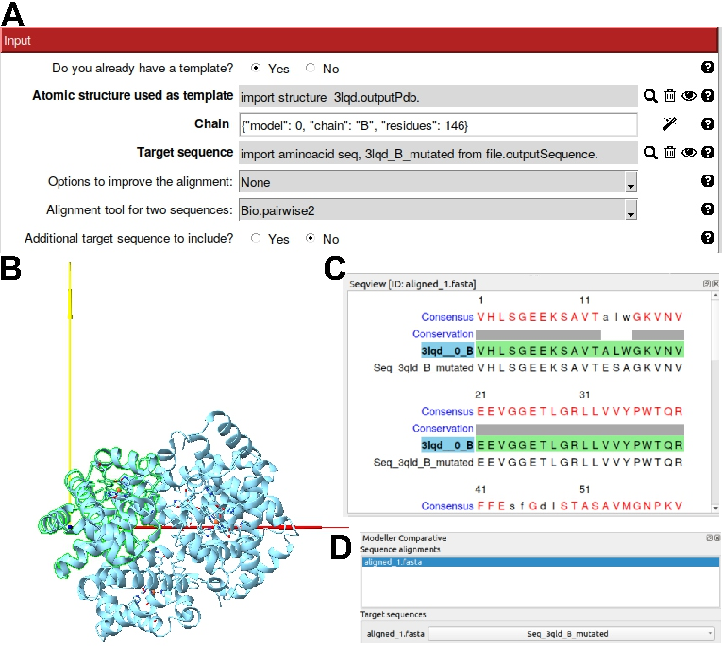
\includegraphics[width=.9\textwidth]{Images_appendix/Fig305.pdf}
                            \caption{(A) Protocol form of \scommand{model from template}. (B) \chimera view of the \iii{template} atomic structure, highlighted in green the \ttt{chain B} selected to perform the modeling. (C) \chimera sequence view panel showing the sequence alignment between the \iii{template} \ttt{chain B} sequence, greeen highlighted, and the \iii{target} sequence. (D) Upper part of the \chimera \ttt{Modeller comparative} panel showing the sequence alignment selected, shown in (C), and the selected \iii{target} sequence.}  
                            \label{fig:app_protocol_seqHomology_2}
                            \end{figure}
                Protocol execution: Complete the protocol form as indicated in \ffigure{fig:app_protocol_seqHomology_2} (A). Follow the general procedure shown above (Protocol execution section). Windows (B) and (C) will appear. Open and complete the \ttt{Modeller Comparative} panel as indicated in (D) and wait for a while. After getting the retrieved models, if you want to select, for example, the \iii{target} model \ttt{\#3.2}, write in the command line:\\
                \ttt{rename \#3.2 id \#4}\\
                \ttt{scipionwrite \#4 prefix model\_3\_2\_}\\
                And \chimera \ttt{Quit} to close the protocol. Visualize your results.
                            
                \item \ttt{Use Case 2: Input atomic structure as template, 2 target sequences, Option ``Additional sequences to align'' to improve the alignment, multichain modeling option in Modeller}\\
                Aim: To model simultaneously two \iii{target} sequences to obtain a multichain model using two chains of a homologous atomic structure as \iii{templates} using other additional sequences than \iii{target} and \iii{template} in the sequence alignment.

 
                            \begin{figure}[H]
                            \centering 
                            \captionsetup{width=.8\linewidth} 
                            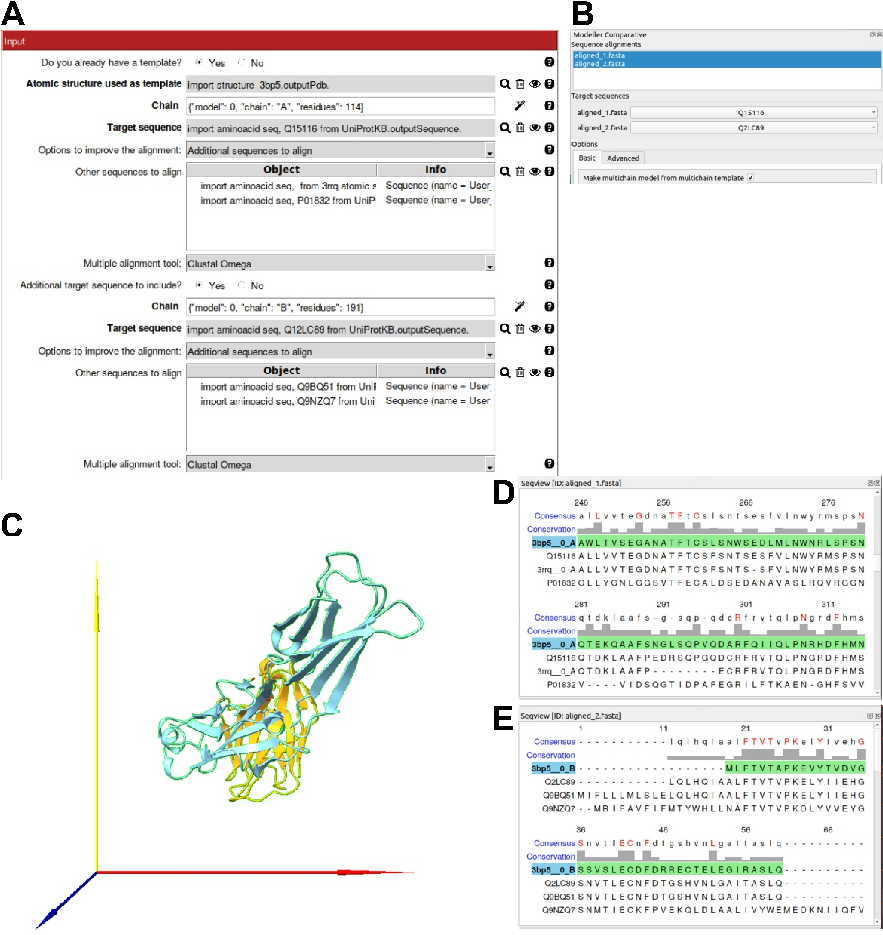
\includegraphics[width=.9\textwidth]{Images_appendix/Fig306.pdf}
                            \caption{(A) Protocol form of \scommand{model from template}. Remark that two additional sequences other than \iii{template} and \iii{target} sequences have been selected to improve both alignments. (B) Upper part of the \chimera \ttt{Modeller comparative} panel showing the two sequence alignment selected, shown in (D) and (E), and the two selected \iii{target} sequences.(C) \chimera view of the \iii{template} atomic structure, highlighted in yellow the \ttt{chain A} and in green the \ttt{chain B} selected to perform the modeling. (D) \chimera sequence view panel showing the sequence alignment between the \iii{template} \ttt{chain A} sequence, greeen highlighted, the \iii{target} sequence (\ttt{Q15116}) and two more additional sequences. (E) \chimera sequence view panel showing the sequence alignment between the \iii{template} \ttt{chain B} sequence, greeen highlighted, the \iii{target} sequence (\ttt{Q12LC89}) and two more additional sequences.}  
                            \label{fig:app_protocol_seqHomology_3}
                            \end{figure}
                            
                 Protocol execution: Complete the protocol form as indicated in \ffigure{fig:app_protocol_seqHomology_3} (A). Follow the general procedure shown above (Protocol execution section). Windows (C), (D) and (E) will appear. Open and complete the \ttt{Modeller Comparative} panel as indicated in (B) and wait for a while. After getting the retrieved models, if you want to select, for example, the \iii{target} model \ttt{\#3.2}, write in the command line:\\
                \ttt{rename \#3.2 id \#4}\\
                \ttt{scipionwrite \#4 prefix model\_3\_2\_}\\
                And \chimera \ttt{Quit} to close the protocol. Visualize your results.
                            
                \item \ttt{Use Case 3: Input atomic structure as template, 2 target sequences, Option ``Provide your own sequence alignment'' to improve the alignment, multichain modeling option in Modeller}\\
                Aim: To model simultaneously two \iii{target} sequences to obtain a multichain model using two chains of a homologous atomic structure as \iii{templates} using your own sequence alignment.

 
                            \begin{figure}[H]
                            \centering 
                            \captionsetup{width=.8\linewidth} 
                            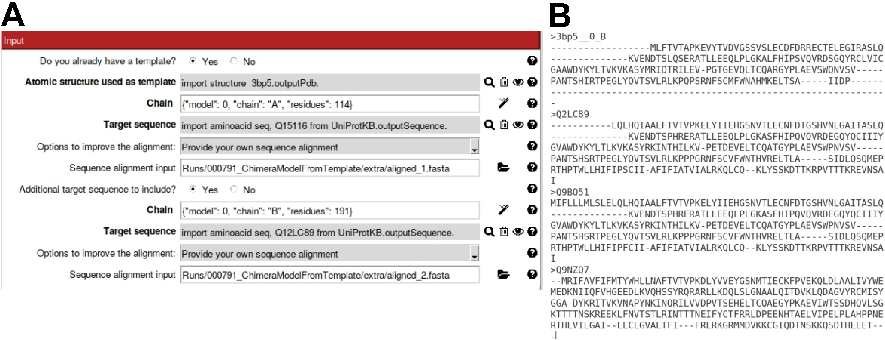
\includegraphics[width=.9\textwidth]{Images_appendix/Fig307.pdf}
                            \caption{(A) Protocol form of \scommand{model from template}. Remark that your own sequence alignment containing the sequences of \iii{template} and \iii{target}, among others, have been selected. (B) Example of sequence alignment in \ttt{fasta} format (file ``aligned\_2.fasta) that includes the \iii{template} \ttt{chain B} sequence, the \iii{target} sequence (\ttt{Q12LC89}) and two more additional sequences.}  
                            \label{fig:app_protocol_seqHomology_4}
                            \end{figure}
                            
                Protocol execution: Complete the protocol form as indicated in \ffigure{fig:app_protocol_seqHomology_4} (A). Follow the general procedure shown above (Protocol execution section). Remark that you already have a sequence alignment file for each \iii{target} saved in your computer. An example can be seen in \ffigure{fig:app_protocol_seqHomology_4} (B). Windows (C), (D) and (E) of previous \ffigure{fig:app_protocol_seqHomology_3} will appear. Open and complete the \ttt{Modeller Comparative} panel as indicated in (B) and wait for a while. After getting the retrieved models, if you want to select, for example, the \iii{target} model {\#3.2}, write in the command line:\\
                \ttt{rename \#3.2 id \#4}\\
                \ttt{scipionwrite \#4 prefix model\_3\_2\_}\\
                And \chimera \ttt{Quit} to close the protocol. Visualize your results.
                            
                \item \ttt{Use Case 4: Input 1 target sequence, PDB searching database}\\
                Aim: To model a \iii{target} sequence without previous information of a possible atomic structure \iii{template}.

 
                            \begin{figure}[H]
                            \centering 
                            \captionsetup{width=.8\linewidth} 
                            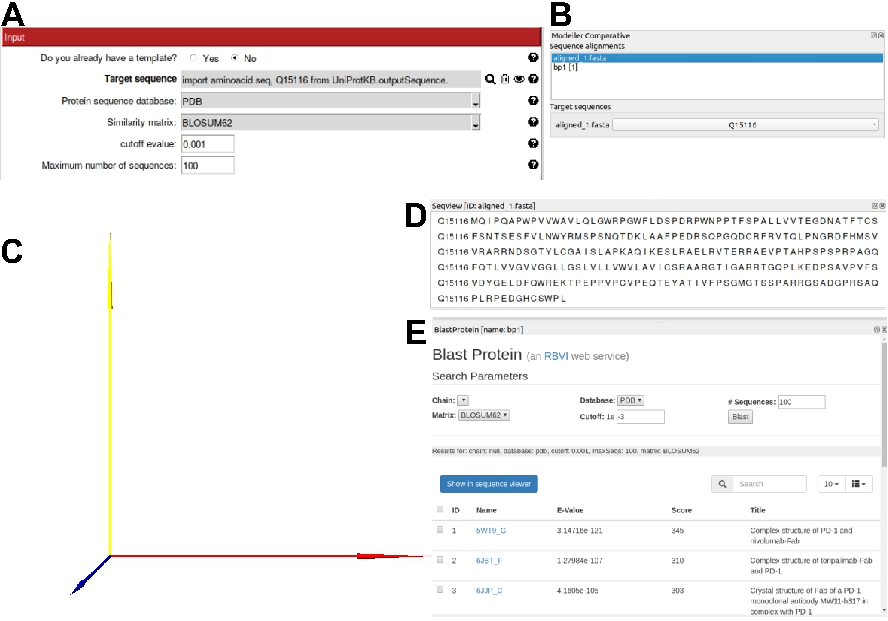
\includegraphics[width=.9\textwidth]{Images_appendix/Fig308.pdf}
                            \caption{(A) Protocol form of \scommand{model from template} that includes the \iii{target} sequence that we'd like to model. (B) Upper part of the \chimera \ttt{Modeller comparative} panel showing the sequence alignment and the \iii{target} sequence selected. (C) \chimera graphics window empty before opening the \iii{template} atomic structure. (D) \chimera sequence view panel showing the \iii{target} sequence. (E) \chimera BlastProtein panel showing the retrieved results from PDB database}
                            \label{fig:app_protocol_seqHomology_5} 
                            \end{figure}
                            
                Protocol execution: Complete the protocol form as indicated in \ffigure{fig:app_protocol_seqHomology_5} (A). Follow the general procedure shown above (Protocol execution section). Remark that in this case there is no \iii{template} atomic structure. Instead, an empty \chimera graphics window will appear (C) together with the \iii{target} sequence that we'd like to model and \ttt{BLASTP} retrieved results (E). Note that it could take some seconds the opening of the \ttt{BlastProtein} panel. Have a look to these results and select one of them as possible \ttt{template} of your \ttt{target} sequence. In this particular case, for example, we are going to choose the first one (\ttt{5WT9}). Open this atomic structure en \chimera by writing in the command line:\\
                \ttt{open 5wt9}\\
                At this point, open the \ttt{Modeller Comparative} panel and complete it as indicated in \ffigure{fig:app_protocol_seqHomology_5} (B). Wait for a while. After getting the retrieved models, if you want to select, for example, the \iii{target} model {\#3.2}, write in the command line:\\
                \ttt{rename \#3.2 id \#4}\\
                \ttt{scipionwrite \#4 prefix model\_3\_2\_}\\
                And \chimera \ttt{Quit} to close the protocol. Visualize your results.
                            
\end{itemize}
